\section{Table Side Recognition}

The points of the table quadrangle are ordered from the upper-left-most point in clockwise order, but this doesn't give
any information on how the sides are ordered. It is unfortunately impossible (or out of my
mathematical capabilities) to find any meaningful geometrical relation between the sides lengths
given the perspective deformations in some cases. The only feature we could exploit was the precence of
holes in the middle of the longer sides. The first operation was to obtain the rotated
rectangles containing the sides of the pool table, with a small width in order to avoid 
keeping in the images unneeded information.\par 
Multiple approaches were tested to distinguish the two types of sides. The first was 
to use features (such as \textit{Harris Corners} or \textit{SIFT}), as intuitively they should appear 
on the holes and not on uniform sides since they should be classified as edges. This didn't
work, as the features and corners detected were spread throughout the 
considered sides most of the as shown in figure \ref{fig:sift}.\par
The next approach was to try \textit{Template Matching} between different segments of the image, more specifically
as the center contains a hole which should make the match significantly worse than
the left and right segments. This did not work for two reasons:
\begin{itemize}
    \item because of the perspective, the hole can appear in a part of the segment of the image that is not the central one;
    \item because of the illumination and small imprecisions on the table segmentation the matching would fail even on the segments which should result similar.
\end{itemize}
Both of these are shown in figure \ref{fig:difficultside}.

\noindent
Ultimately, the way to recognize the sides was the following:
\begin{enumerate}
    \item apply the Canny tranform on the initial image;
    \item extract the rectangles from the image;
    \item rotate the rectangles so that they are all horizontal;
    \item apply sobel on the x-axis shown in image \ref{fig:sidestabol};
    \item sum over the contributions on the middle two quarters (to avoid considering the corner holes) of the rectangles normalized over the number of pixels contained in each;
    \item determine the longer sides by the highest contributions.
\end{enumerate}
This works because of the nature of the edges on the sides: on shorter sides there
are mostly parallel lines, instead on longer ones there are strong edges orthogonal to the direction of the sides given by the holes.

\begin{figure}
    \centering
    \begin{subfigure}[b]{\textwidth}
    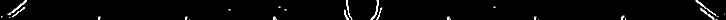
\includegraphics[width=\textwidth]{./imgs/sobel_long_side.png}
    \caption{Processed rectangle of a long side}\par
    \end{subfigure}\vspace{10pt}
    \begin{subfigure}[b]{\textwidth}
    
\includegraphics[width=\textwidth]{./imgs/sobel_short_side.png}
    \caption{Processed rectangle of a short side}
    \end{subfigure}
    \caption{Output of the processing of the sides}
    \label{fig:sidestabol}
\end{figure}

\vspace{20pt}

\begin{figure}
    \centering
    \begin{subfigure}[b]{\textwidth}
    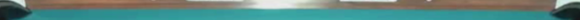
\includegraphics[width=\textwidth]{./imgs/bad_side_illumination_change.png}
    \caption{extreme illumination change in the  center of the side}\par
    \end{subfigure}\vspace{10pt}
    \begin{subfigure}[b]{\textwidth}
    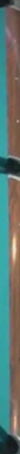
\includegraphics[angle=90, width=\textwidth]{./imgs/bad_side_warp.png}
    \caption{not centered hole}
    \end{subfigure}
    \caption{Examples of difficulties in side recognition}
    \label{fig:difficultside}
\end{figure}
\begin{figure}
    \centering
    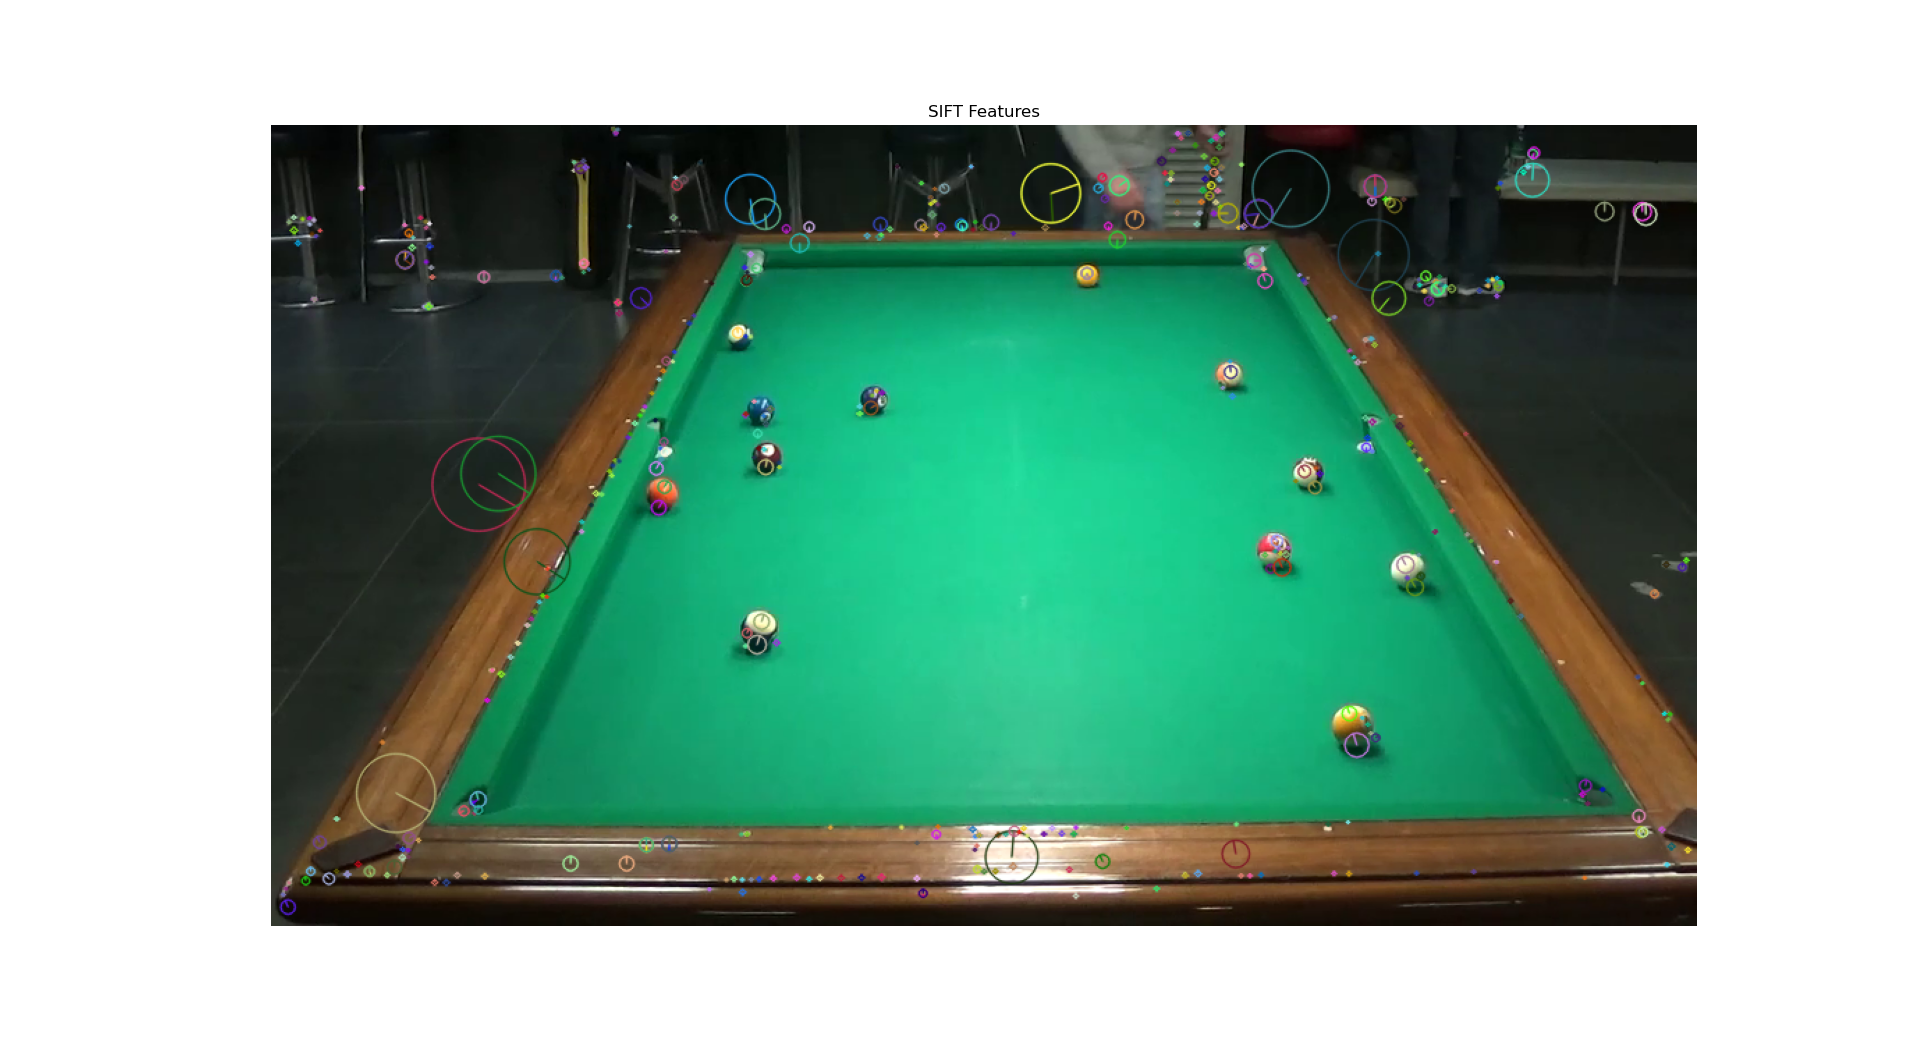
\includegraphics[width=\textwidth]{./imgs/sift.png}
    \caption{Sift features in a sample image}
    \label{fig:sift}
\end{figure}
